% Created 2020-09-09 Wed 15:23
% Intended LaTeX compiler: pdflatex
\documentclass[nobib]{tufte-handout}
                                  \usepackage[svgnames]{xcolor}
\usepackage{times}
\usepackage{hyperref}
\usepackage{url}
\makeatletter
\renewcommand{\maketitle}{%
\newpage
\global\@topnum\z@% prevent floats from being placed at the top of the page
\begingroup
\setlength{\parindent}{0pt}%
\setlength{\parskip}{4pt}%
{\Large\bf\@title}\par
{\normalfont\normalsize\@author}\par
\endgroup
\thispagestyle{plain}% suppress the running head
\tuftebreak% add some space before the text begins
\@afterindentfalse\@afterheading% suppress indentation of the next paragraph
}
% Paragraph indentation and separation for normal text
\renewcommand{\@tufte@reset@par}{%
\setlength{\RaggedRightParindent}{0pt}%
\setlength{\JustifyingParindent}{0pt}%
\setlength{\parindent}{0pt}%
\setlength{\parskip}{0.5pc}%
}
\@tufte@reset@par
\makeatother
\fancyhead[RE,RO]{\newlinetospace{\color{gray}\plaintitle}\quad\thepage}
\usepackage{amsmath}
\usepackage{amssymb}
\usepackage{mathtools}
\usepackage{colortbl}
\usepackage{cleveref}
\usepackage{svg}
\usepackage{bm}
\usepackage{booktabs}
\usepackage{multirow}
\usepackage{grffile}
\usepackage{pgfplots}
\usepackage[caption=false]{subfig}
\usepackage{wrapfig}
\usepackage{microtype}
\usepackage{xspace}
\pgfplotsset{compat=newest}
\usepackage{tikz}
\usetikzlibrary{positioning,quotes}
\usepackage[style=authoryear,backend=bibtex,natbib,maxcitenames=2,doi=false]{biblatex}
\addbibresource{./references.bib}
\hypersetup{
colorlinks = true,
allcolors = {DarkBlue}
}
\captionsetup{labelfont=bf}
\renewcommand{\vec}[1]{\bm{#1}}
\newcommand{\AR}{\text{AR}}
\newcommand{\bAR}{\ensuremath{\beta}\text{-AR}\xspace}
\newcommand{\Set}[1]{\mathcal{#1}}
\newcommand{\risk}{\mathcal{R}}
\newcommand{\foi}{\lambda}
\newcommand{\E}{\mathbb{E}}
\newcommand{\todo}[1]{{\color{red} #1}}
\author{Matthew Le, Mark Ibrahim, Levent Sagun, Timothee Lacroix, \\  Maximilian Nickel \\  Facebook AI Research}
\date{}
\title{Neural Relational Autoregression \\  for High-Resolution COVID-19 Forecasting}
\hypersetup{
 pdfauthor={Matthew Le, Mark Ibrahim, Levent Sagun, Timothee Lacroix, \\  Maximilian Nickel \\  Facebook AI Research},
 pdftitle={Neural Relational Autoregression \\  for High-Resolution COVID-19 Forecasting},
 pdfkeywords={},
 pdfsubject={},
 pdfcreator={Emacs 26.3 (Org mode 9.4)}, 
 pdflang={English}}
\begin{document}

\maketitle
\marginnote[-2.15em]{Corresponding author: Maximilian Nickel \texttt{maxn@fb.com}}

\begin{abstract}
Forecasting COVID-19 poses unique challenges due to the novelty of the disease,
its unknown characteristics, and substantial but varying interventions to reduce
its spread. To improve the quality and robustness of forecasts, we propose a new
method which aims to disentangle region-specific factors -- such as
demographics, enacted policies, and mobility -- from disease-inherent factors
that influence its spread. For this purpose, we combine recurrent neural
networks with a vector autoregressive model and train the joint model with a
specific regularization scheme that increases the coupling between regions. This
approach is akin to inducing Granger causality in the autoregressive part and
allows us to train high-resolution models by borrowing statistical strength
across regions. In our experiments, we observe that our method achieves strong
performance in predicting the spread of COVID-19 when compared to
state-of-the-art forecasts.
\end{abstract}

\section{Introduction}
\label{sec:orgae0e6ce}
Modeling the spread of COVID-19 at a high spatial and temporal resolution (i.e.,
confirmed cases at county or admin-3 level) has become an important task in the
public health response to the disease. For instance, accurate county-level
forecasts are not only central to monitor the state of the pandemic but are also
important to efficiently allocate scarce resources such as ventilators, personal
protective equipment, and ICU beds; and to make progress towards efficient early
detection systems.

\begin{marginfigure}[-45em]
\hspace{-2.5em}%
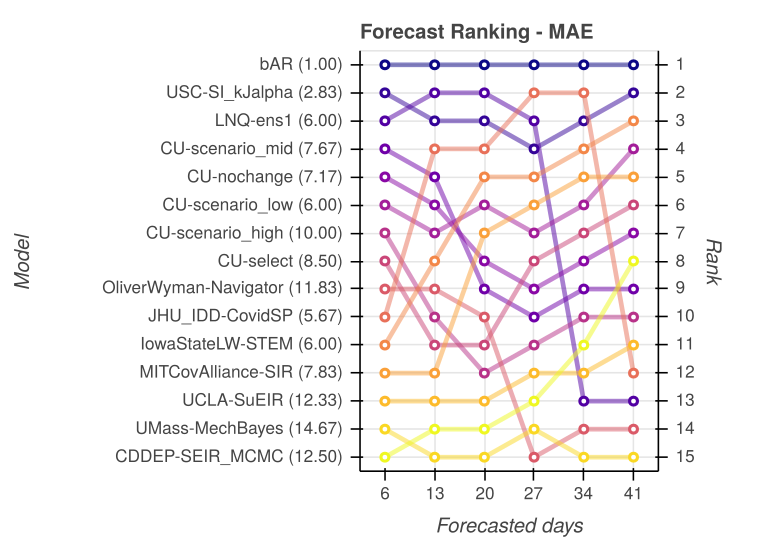
\includegraphics[width=1.3\columnwidth]{img/us_rank_mae.png}
\caption{Ranking of county-level forecasts by average MAE over various forecast horizons. The proposed neural relational autoregressive model (\bAR) shows strong performance over all horizons when compared to state-of-the-art forecasts. Mean rank over all horizons in parentheses.}
\label{fig:ranking-covidhub-mae}
\end{marginfigure}


\begin{marginfigure}[-7em]

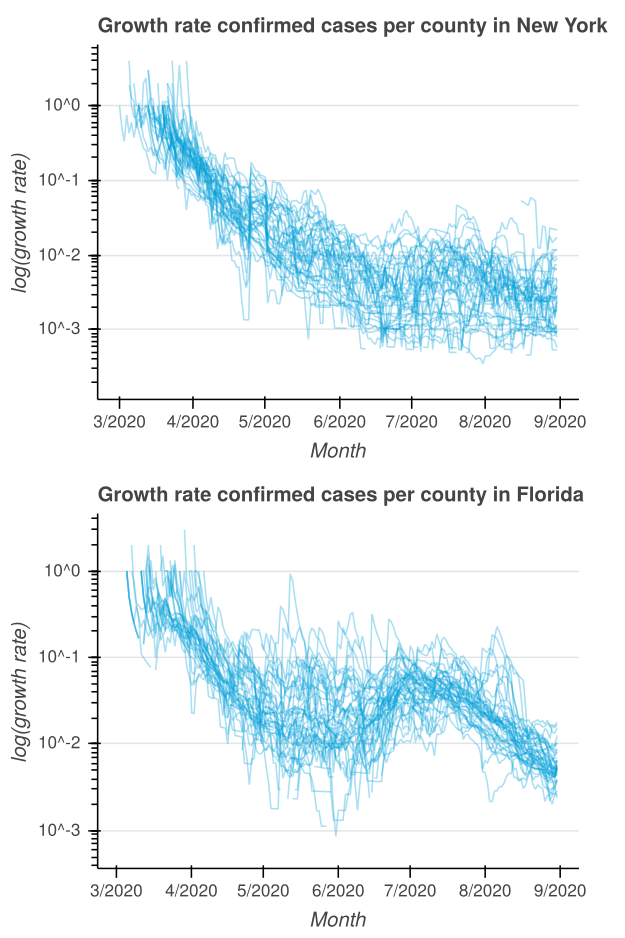
\includegraphics[width=\columnwidth]{img/growth_example.png}
\caption{\label{fig:county-variability}Variability of growth in confirmed cases per region over time}
\end{marginfigure}

However, forecasting COVID-19 poses unique challenges -- in particular when
considering confirmed cases at high spatial resolution. Although there has been
considerable progress towards understanding the spread of the disease, there
still exists only limited data and knowledge about important factors that
influence its spread. This is only exacerbated by the naturally larger
noise-levels in county-level data as compared to more highly aggregated state-level
data. Due to the global nature of COVID-19, the available data is also
distributed among regions with very different properties, many of which may
affect its spread. This includes, for instance, demographics and population
densities, enacted policies, adherence to those policies, mobility patterns, and
geographic features such as temperature. In addition, testing and reporting can
change considerably across regions and time. All these factors lead to
considerable variablity (see also \Cref{fig:county-variability}) and uncertainty in
the data and makes reliable forecasts at high spatial resolution difficult.

To alleviate these issues, we propose a new method for predicting the spread of
COVID-19 by combining recurrent neural networks with a vector autoregressive
model and a specific regularization relational scheme. Our approach is motivated
by two main aspects: First, we seek to develop an end-to-end differentiable
model, as this allows us to make efficient use of the limited available data
while also enabling us to estimate parameters of powerful models that can capture
the large variability of cases across locations and time. However, while such
flexible models are needed to account for all possible influencing factors there
is little data to estimate them reliably and without overfitting. For this
reason, we seek, second, to disentangle region- and time-specific factors from
disease-inherent factors that influence its spread. This allows us to borrow
statistical strength between regions by coupling their predictions -- based on
the assumption that once a model has correctly accounted for region-specific
dynamics, information about the spread of the disease in region \(j\) should
therefore also help to improve predictions for a related region \(i\). This
approach is akin to using \emph{Granger causality} as an inductive bias to improve
forecast quality and robustness.

Compared to existing state-of-the-art forecasting models, our method takes a
highly data-driven approach with fewer modeling assumptions as, for instance, in
very detailed compartmental models. As such we see our approach as complementary
to existing models which provides strong forecasting performance at the cost of
reduced interpretability.


\section{Neural Relational Autoregression}
\label{sec:org914e4a2}
We consider the forecasting of \(m\) time series that are different realizations
of the same underlying disease process. Let \({\Set{Y} = \{(y_i^1, \ldots,
y_i^T)\}_{i=1}^m}\) denote the observed case counts where \(i\) indexes locations
and where \(T\) denotes the maximum observation time. Furthermore, let
\(\Set{Y}(\tau) = \{(y_i^t : t \leq \tau)\}_{i=1}^m\) denote the set of all
observed case counts up to time \(\tau \leq T\). We then model the case counts as
random variables
\begin{equation*}
    Y^{t+1}_i\ |\ \Set{Y}(t) \sim f(\foi_i^t)
\end{equation*}
where \(\foi_i^{t}\) denotes the \emph{force of infection}\sidenote[]{Given \(y^t_i\) infected
individuals, the force of infection (or hazard) models the probability that a
susceptible individual at time \(t\) will become infected by time \(t+1\)} at time
\(t\) in location \(i\) and where \(f(x)\) denotes a probability distribution with
parameter \(x\) (e.g., a Poisson or Negative Binomial distribution).

Due to the different interventions during the course of the epidemic, we regard
\(\Set{Y}\) as a time-varying process that is influenced by external factors such
as policies, mobility, etc. For this reason, we decompose \(\foi_i^t\) into a
time-specific component \(\beta_i^t\) and a time-indepedent component
\(\foi_i\) such that
\begin{align*}
\foi_i^t = \beta_i^t \foi_i \quad\text{where}\quad \beta_i^t \in [0, 1],\, \foi_i > 0
\end{align*}

Hence, \(\beta_i^t\) can be understood as a dampening factor of the underlying
force of infection which models the effect of interventions and depends on time
and location. While some influencing factors for the evolution of \(\beta_i^t\)
might be known (e.g., mobility, population density, etc.), we assume that the
full set of influencing factors is unknown and will regard \(\beta_i^t\)
as a latent variable.

Using this decomposition, we then model the time-independent force of
infection as a autoregressive model of order \(p\),\sidenote[]{AR models
where \[Y_i^{t+1}\ |\ \Set{Y}(t) \sim \text{Poisson}(\foi_i^t)\] can be
interpreted as approximations of Reed-Frost chain binomial SIR models. For a
detailed discussion see \citep{bauer2018stratified}.} i.e.,
\begin{align}
    \text{AR}(p): \foi_i = \sum_{\ell=0}^{p-1} w^\ell y_i^{t - \ell} \label{eq:foi-ar}
\end{align}
where \(\{w^\ell > 0\}_{l=0}^{p-1}\) are the parameters of the model which are
shared across locations \(i\). For the time-depdendent dampening \(\beta_i^t\) we
employ recurrent neural networks (RNNs) such that
\begin{align}
    \text{RNN}: \beta_i^t = f_\theta(\{x_i^k\}_{k=0}^t) \label{eq:rnn}
\end{align}
where \(\theta\) are the parameters of the network which are again shared across
locations and where \(\{x_i^k\}_{k=0}^t\) denote observed input features to the
RNN (e.g., mobility in location \(i\) at time \(k\)). Although an RNN as in
\Cref{eq:rnn} has enough capacity to model the evolution of \(\beta_i^t\), the
limited data about the spread of COVID-19 makes it challenging to estimate its
parameters without overfitting. We seek therefore an inductive bias which allows
us to estimate \(\beta_i^t\) from few observations.

\subsection{Relational Inductive Bias}
\label{sec:orge63875c}

Since all regions are affected by the same underlying process, we assume that
information about the spread in region \(i\) should also help to predict the
spread in region \(j\) -- once we have accounted for time- and location-dependent
dynamics. A good model of \(\beta_i^t\) should therefore help to improve the
predictions of \(y_i^{t+1} / \beta_i^t\) from cases in other regions \(y_j^t\). We
interpret this inductive bias akin to Granger causality\sidenote[]{Granger causality is
defined as follows: Let \({X^t=\{X_t\}_{i=1}^t}\), \({Y^t=\{Y_t\}_{i=1}^t}\),
\({Z^t=\{Z_t\}_{i=1}^t}\) denote stochastic processes and let \(L\) denote a loss
function. Furthermore, let \[\risk(Y^{t+1} | Y^t, Z^t) = \E(L(Y_{t+1}, f(Y^t,
Z^t)))\] denote the expected loss (risk) of a predictor \(f\). We then say \(X\)
\emph{Granger-causes} \(Y\) if its inclusion in the predictor significantly improves
the forecast, i.e., if \[ \risk(Y^{t+1} | Y^t, X^t, Z^t) \ll \risk(Y^{t+1} |
Y^t, Z^t) \]} and extend \Cref{eq:foi-ar} to a \emph{vector autoregressive} model where
it is known that Granger causality is directly linked to its coefficients. In
particular, let
\begin{equation} \text{VAR}(p): \foi_i =
\sum_{\ell=0}^{p-1} \sum_{j=1}^m w_{ij}^\ell y_j^{t - \ell}
\end{equation}
be a vector autoregressive model of order \(p\). \emph{A time series \(y_j\) is then
Granger-causing \(y_i\) if and only if \(w_{ij} \neq 0\)} \citep{Seth2007granger}. For
causal discovery, coefficients \(w_{ij}\) are therefore often
\(\ell_1\)-regularized. Here, we take the opposite approach and seek solutions
in which as many time-series as possible can be considered Granger-causal
related. However, we do not force all time series to be related since this is
likely an unrealistic constraint. Instead, we assume \(\forall i \neq j : w_{ij}\)
are drawn from a logit-normal distribution \citep{atchison1980logistic}, what
allows us to specify a prior on the proportion of related and unrelated time
series.

\begin{marginfigure}[2em]
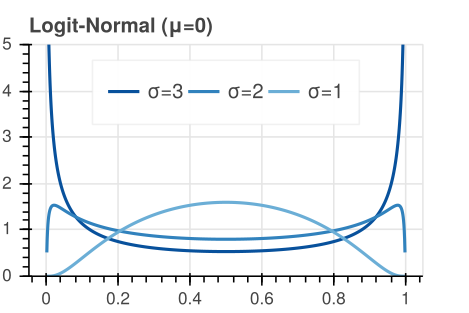
\includegraphics[width=\columnwidth]{img/logit_normal_0.png}
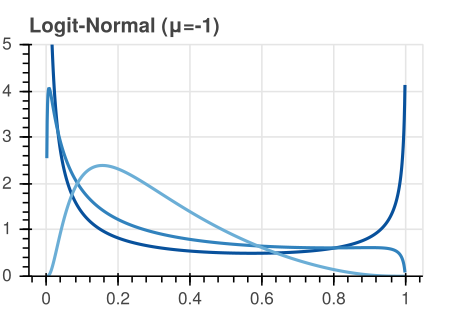
\includegraphics[width=\columnwidth]{img/logit_normal_-1.png}
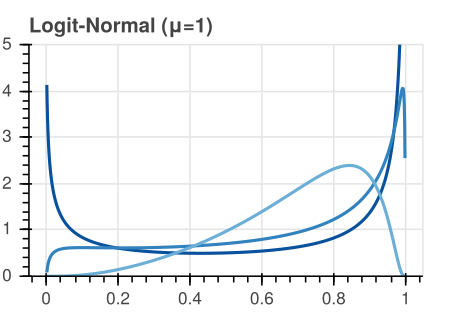
\includegraphics[width=\columnwidth]{img/logit_normal_1.png}
\caption{The Logit-Normal distribution is a probability distribution of a random variable whose logit has a normal distribution, i.e., $\phi(\mathcal{N}(\mu, \sigma))$.}
\end{marginfigure}

In particular, let \(\phi(\cdot)\) denote the logistic function, let \({\forall i
\neq j : w_{ij} = \phi(\alpha_{ij})}\), and let \(\mathcal{N}(\mu, \sigma^2)\)
denote the Normal distribution with mean \(\mu\) and variance \(\sigma^2\). Putting
everything together, we then model the full \emph{time-varying} force of infection as
\begin{align}
\bAR(p): \quad \foi^{t+1}_i & =
\beta_i^t \sum_{\ell=0}^{p-1}\sum_{j=1}^m w_{ij}^\ell y_j^{t - \ell} \label{eq:beta-ar} \\
    \alpha_{ij} & \sim \mathcal{N}(\mu, \sigma^2) \quad \forall i \neq j \notag
\end{align}
Hence, the \(\bAR\) model consists of a standard \AR\xspace component (\(w_{ii} > 0\)) and
a relational component (\(w_{ij} \in [0, 1]\)) which aims to couple the different
regions. The number of non-zero entries in the ``adjacency matrix'' \(w_{ij}\) can
then be controlled through the logit-normal prior.

\subsection{Accounting for Overdispersion}
\label{sec:org8286d6d}
Count data such as confirmed cases is naturally modeled using Poisson
distributions. However, COVID-19 case counts exhibit substantial overdispersion,
i.e., the variance of the observed counts can significantly exceed their mean
(e.g., see \cref{fig:dispersion}). For this
reason, we will model case counts with Negative Binomial distributions what
allows us to account for varying degrees of overdispersion. Specifically, we set
\begin{align*}
    y^{t+1}_{i} & \sim \text{NB}(\foi_i^{t}, \nu_i)
\end{align*}
where \(\foi^t_i\) and \(\nu_i\) are mean and dispersion parameter of the
distribution and \(\foi^t_i\) is modeled using the \bAR model of \cref{eq:beta-ar}. The
likelihood function in \cref{eq:objective} is then of the form
\begin{equation*}
p_\theta(y) = \frac{\Gamma(y + \nu)}{y!\Gamma(\nu)}\left(\frac{\mu}{\mu +\nu}\right)^{y}\left(1 + \frac{\mu}{\nu}\right)^{-\nu}
\quad \mu > 0, \nu > 0
\end{equation*}

\begin{marginfigure}[5em]
\hspace{0em}%
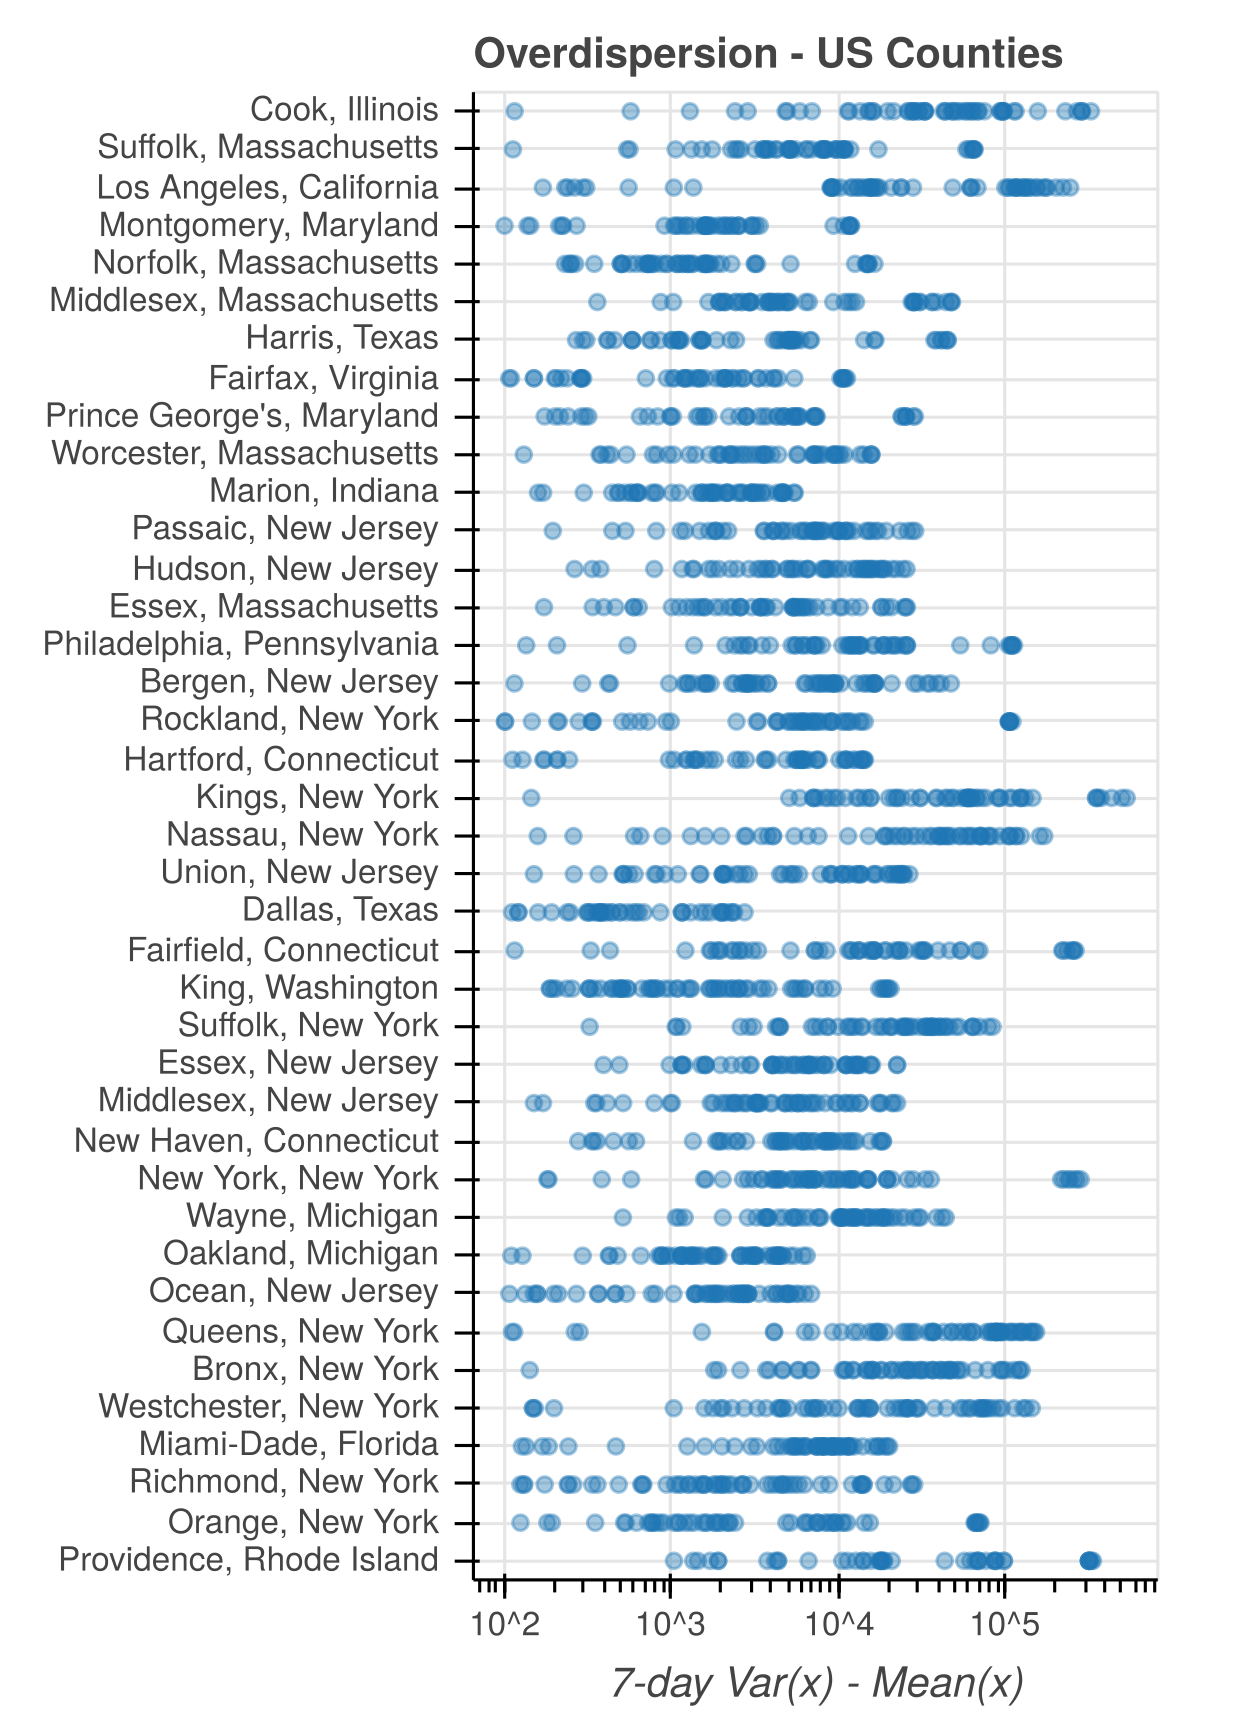
\includegraphics[width=\columnwidth]{img/overdispersion_counties.png}
\caption{Overdispersion of daily case counts in US states and counties with most number of cases.}
\label{fig:dispersion}
\end{marginfigure}

\subsection{Parameter Estimation and Implementation Details}
\label{sec:org9e86a8e}
To estimate the parameters of the model, we regularize the
model log-likelihood such that \(w_{ij}\) is drawn from a logit-normal
distribution with location \(\mu\) and scale \(\sigma\). Let \(\theta\) denote
the model parameters (i.e., \(\alpha_{ij}\) as well as parameters of the RNN).
and let \(p_\theta(y)\) denote the likelihood function of the \(\bAR\)
model. Furthermore, let \(q\) denote the prior normal
distribution for \(\alpha_{ij}\). We then maximize the regularized log-likelihood
\begin{equation}
\max_{\theta}\sum_y\log p_\theta(y) + \sum_{ij} \log q(\alpha_{ij}\,|\,\mu,\sigma). \label{eq:objective}
\end{equation}
We regard \(\mu, \sigma > 0\) as hyperparameters which allow us to control the
ratio of related and unrelated time series.

Since \Cref{eq:objective} is end-to-end differentiable we can jointly estimate the
parameters of the entire model using gradient-based optimization. We compute
gradients via automatic differentiation using the PyTorch framework
\citep{paszke2019pytorch}. To maximize \Cref{eq:objective} we then use the stochastic
optimization method AdamW \citep{loshchilov2018decoupled} where we decouple the
updates of the normally distributed parameters \(\alpha_{ij}\) from the adaptive
updates of the remaining parameters.

\section{Results}
\label{sec:org7d76cd4}
In the following, we evaluate the forecast quality of our method compared to
multiple state-of-the-art forecasts for confirmed cases on
county-level. All comparison forecasts are collected from the COVID-19 Forecast
Hub\sidenote[]{\url{https://github.com/reichlab/covid19-forecast-hub}} as submitted by
the respective teams. The COVID-19 Forecast Hub features county-level forecasts
from July 5th onwards and we selected those models for which at least 10 forecasts
where available since then. The full list of comparison forecasts is shown in
\Cref{tab:forecasts}.

\begin{table*}[t]
\small
\centering
\begin{tabular}{lll}
\toprule
\bf Group & \bf Model \\
\midrule
Center for Disease Dynamics, Economics \& Policy & \it CDDP-SEIR\_MCMC & \citep{cddep_seir_mcmc} \\
Columbia University & \it CU-* & \citep{forecasts/columbia} \\
COVID Alliance at MIT & \it MITCovAlliance-SIR & \citep{baek2020limits} \\
Iowa State University Lily Wang Research Group & \it IowaStateLW-STEM & \citep{wang2020spatiotemporal} \\
Johns Hopkins ID Dynamics COVID-19 Working Group & \it JHU-IDD\_CovidSP & \citep{forecasts/jhu_idd_covidsp} \\
LockNQuay & \it LNQ-ens1 & \citep{forecasts/lnq_ens1} \\
Oliver Wyman & \it Pandemic Navigator & \citep{forecasts/oliver_wyman} \\
UCLA Statistical Machine Learning Lab & \it UCLA-SuEIR & \citep{forecasts/Zou2020.05.24.20111989} \\
University of Southern California Data Science Lab & \it USC-SI\_kJalpha & \citep{srivastava2020fast} \\
University of Massachussets Amherst & \it UMass-MechBayes & \citep{forecasts/umass_mechbayes} \\
\bottomrule
\end{tabular}
\vspace*{2em}
\caption{Forecasting models for confirmed cases on county-level.\label{tab:forecasts}}
\end{table*}

\paragraph{Forecast setup and model selection} To compute forecasts for the
different dates in the test set, we use the following fully automated model
selection scheme: For each forecast date \(d\), we perform cross-validation by
holding out additional 21 days of validation data and train the model on the
remaining data. We then select the best hyperparameters as measured by RMSE on
the validation set and retrain the whole model with those hyperparameters on the
combined training and validation set to compute the final forecast. When
computing the forecasts, we hold all additional input data (e.g., symptom
survey, mobility, weather, etc.) constant after the last observed day
\(d\).\sidenote[]{This setting places natural limits on the duration of the forecasting
horizon. We reserve the joint forecasting of cases and covariates -- what could
extend the horizon -- for future work.}. For all training details of the model,
please see the supplementary material.


\paragraph{Input data} As input features for \bAR, we use multiple data sources as listed in
\Cref{tab:data-sources}. Confirmed cases enter the model only in the autoregressive
part. All other covariates enter the model only as input features for the
time-varying \(\beta\)-part. For cases and weather data, we use the preprocessed data
from the Google COVID-19 Open Data repository \citep{data/Wahltinez2020}.

\begin{table*}[t]
\small
\centering
\begin{tabular}{lll}
\toprule
\bf Dataset & \bf Source & \bf Resolution \\
\midrule
Confirmed Cases &  \citet{data/nytimes_cases} &  County \\
& \multicolumn{2}{l}{\it Confirmed cases based on reports from state \& local health agencies} \\
\midrule
Symptom Survey & \citet{data/fb_symptom_survey} &  County, State \\
& \multicolumn{2}{l}{\it Prevalence of COVID-like symptoms from self-reported surveys} \\
\midrule
Movement Range Maps &  \citet{data/fb_movement_range} &  County, State \\
& \multicolumn{2}{l}{\it Mobility metrics related to physical distancing measures} \\
& \multicolumn{2}{l}{\it (change in movement and staying put)} \\
\midrule
Community Mobility & \citet{data/google_mobility} &  County, State \\
& \multicolumn{2}{l}{\it Movement trends across different categories of places} \\
& \multicolumn{2}{l}{\it (retail and recreation, groceries and pharmacies, etc.)} \\
\midrule
Doctor visits & CMU COVIDcast \citep{data/covidcast} & County, State \\
& \multicolumn{2}{l}{Percentage of COVID-related doctor’s visits in a given location} \\
\midrule
Testing &  \citet{data/covidtracking} & State \\
& \multicolumn{2}{l}{\it Total number of COVID PCR tests per state} \\
\midrule
Weather & NOAA GHCN \citep{data/menne2012overview} &  County \\
& \multicolumn{2}{l}{\it Average, minimum, maximum temperature \& rainfall per county} \\
\bottomrule
\end{tabular}
\vspace*{2em}
\caption{Data sources for \bAR.\label{tab:data-sources}}
\end{table*}

\paragraph{Forecast evaluation} \Cref{fig:mae-covidhub} shows the forecast
quality as measured by MAE for multiple forecast horizons.\sidenote[]{MAE numbers are computed in accordance with \url{https://github.com/youyanggu/covid19-forecast-hub-evaluation}} It can be seen that
the proposed \bAR models shows a consistently strong performance and is for all
forecasting dates and horizons either the best model or among the best.
\Cref{fig:ranking-covidhub-mae}, which shows the ranking of all models by the
average MAE for each forecast horizon, further illustrates this property. It can
be seen that \bAR model is consistently ranked first over all horizons.
Furthermore, other models show much larger variability in their performance.

\begin{figure}[htbp]
\centering
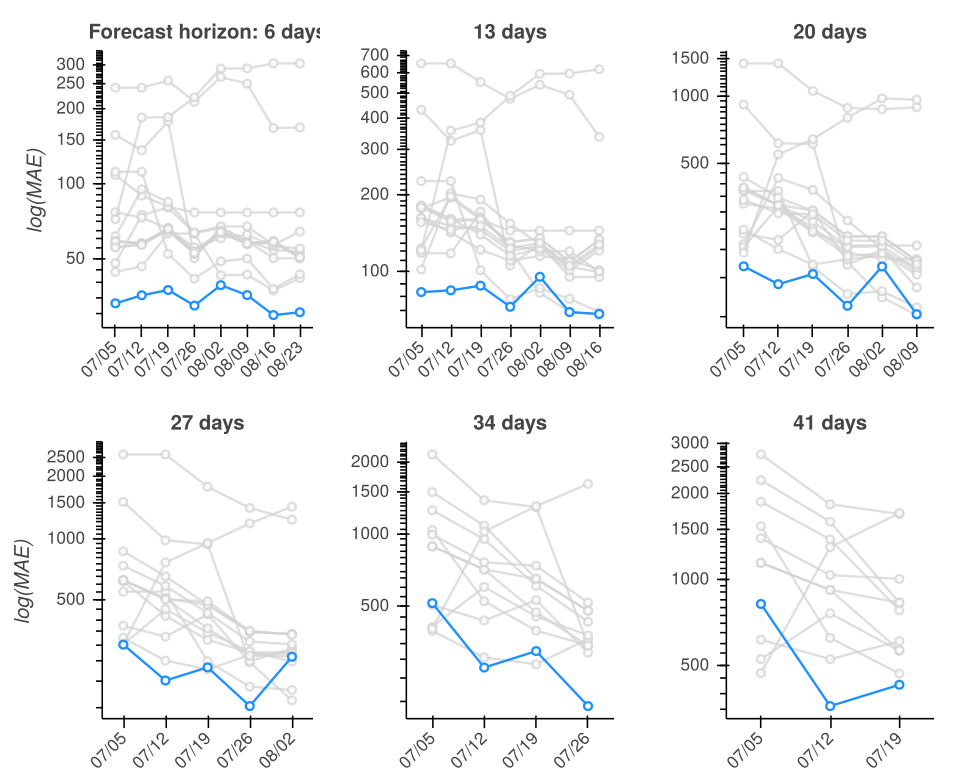
\includegraphics[width=\columnwidth]{img/us_mae/us_mae.png}
\caption{\label{fig:mae-covidhub}Comparison of \bAR model (blue) to 15 county-level models from COVID-19 forecast hub (gray). Forecast quality is measured in MAE (log-scale). For similar analysis using RMSE please see the supplementary material.}
\end{figure}


To also evaluate the performance of our model on days prior to July 5th, we
compare to forecasts of Google Cloud AI \citep{arik2020interpretable} and Columbia
University \citep{forecasts/columbia} which provide county-level forecasts of
confirmed cases from May 11th to June 27th. \Cref{fig:mae-google} shows the average
MAE over all counties for 7 and 14 day forecasts for these models.\sidenote[]{For this
comparison, average MAE is computed as described in \citep{arik2020interpretable}}
It can be seen that the \bAR model shows again consistently strong performance on these
earlier days and is typically ranked first for both 7 and 14 day forecasts.

\begin{figure*}
\centering
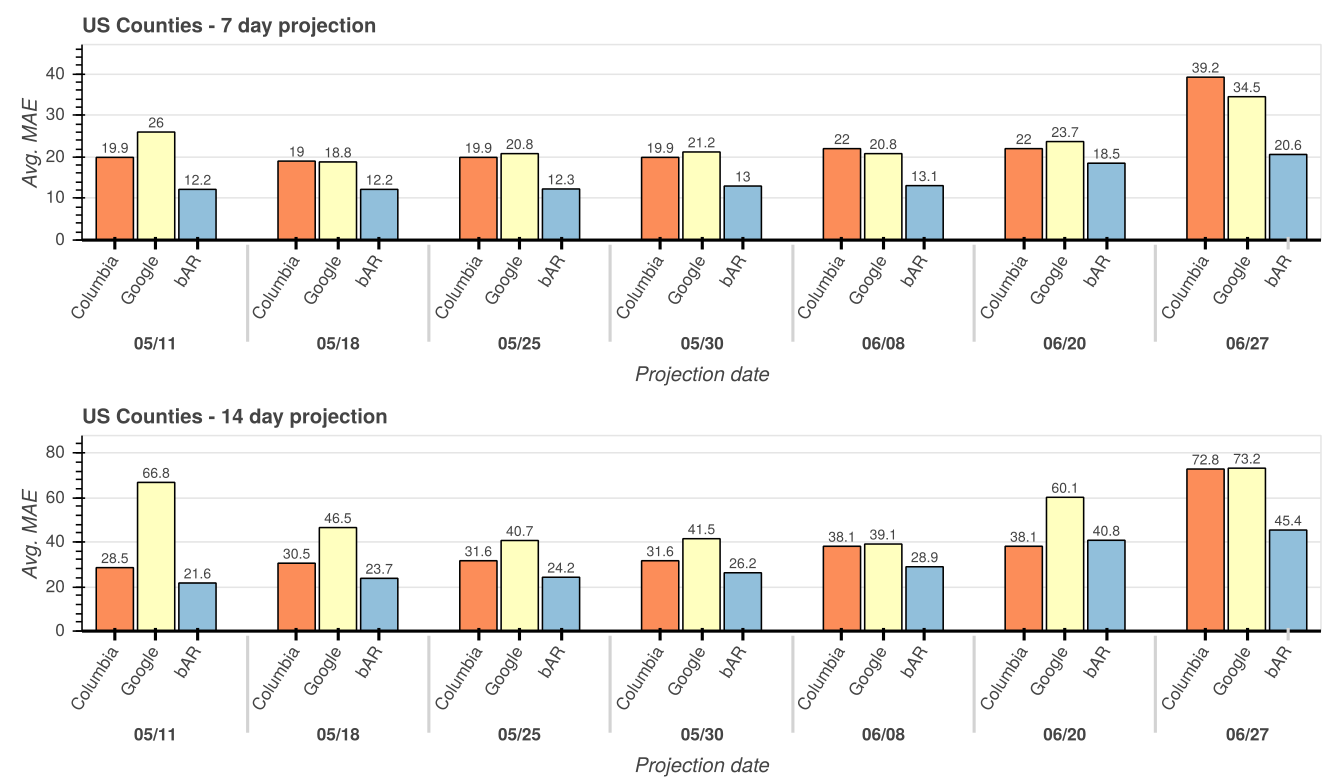
\includegraphics[width=\columnwidth]{img/counties_bar_mae.png}
\caption{\label{fig:mae-google}Comparions of \bAR model to forecasts from Google Cloud AI and Columbia for 7 and 14 day horizons. Forecast quality is measured in MAE. For a similar analysis using RMSE please see the supplementary material.}
\end{figure*}

\paragraph{Ablations} In addition to comparisons to state-of-the-art
county-level forecasts, we also evaluate the contributions of different aspects
of our model. First, we test the effect of the relational autoregressive part.
For this purpose, we trained additional models were we disabled the relational
part (by setting \(\forall i \neq j: w_{ij} = 0\)) and compared their forecasts to
the full model of \Cref{eq:beta-ar}. To measure the relative improvement of the
full model over the non-relational model, we compute then the relative error of
both models, e.g.,
\begin{equation*}
    \text{Relative Mean Absolute Error} = \frac{\text{MAE}_{\text{full}}}{\text{MAE}_\text{non-relational}}
\end{equation*}
It can be seen from \Cref{fig:quality-ratio} that full model offers substantial
improvements over the non-relational model as the relative forecast quality
grows exponentially with the forecasting horizon. While the non-relational model
can offer acceptable forecast for horizons of 1-2 days, it quickly deteriorates
with larger horizons. This show the importance of the relational component for
disentangling the different growth factors and learning high quality models.

\begin{marginfigure}[-30em]

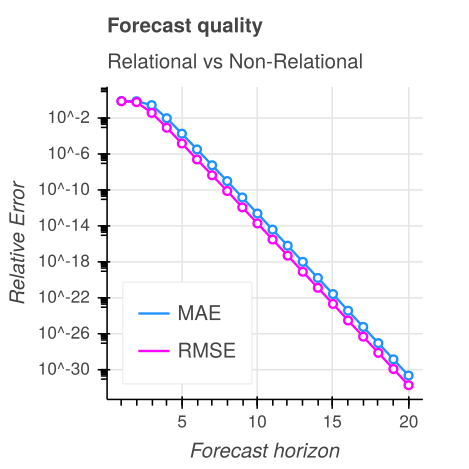
\includegraphics[width=\columnwidth]{img/quality_ratio.png}
\caption{\label{fig:quality-ratio}Relative Error (MAE and RMSE) of the fully relational \bAR model compared to a non-relational variant.}
\end{marginfigure}

\begin{figure}[htbp]
\centering
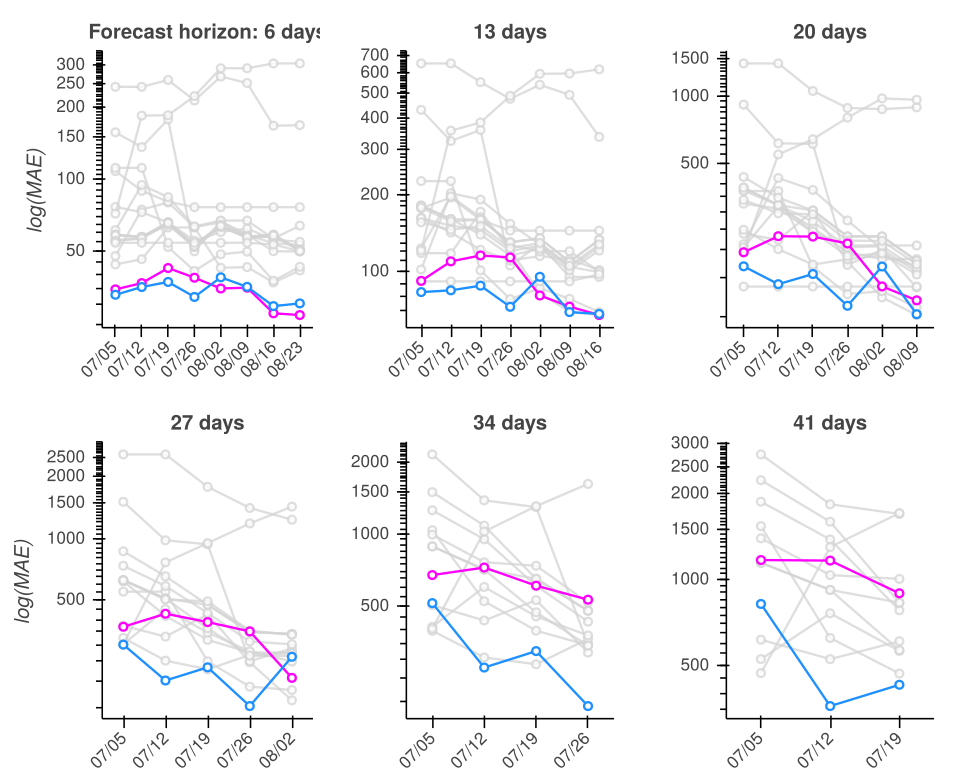
\includegraphics[width=\columnwidth]{img/us_mae_granger_ablation/us_mae_granger_ablation.png}
\caption{\label{fig:mae-covidhub-granger}Comparison of \bAR model with (blue) and without (magenta) Granger regularization. Forecast quality is measured in MAE.}
\end{figure}

In addition to the non-relational component, we also evaluated the contributions
of the logit-normal regularization method. For this purpose, we trained a model
where we explicitly set the reqularization parameter \(\sigma = 0\). We then
compare the forecast quality to the standard model where the regularization
parameter has been selected via cross-validation. \Cref{fig:mae-covidhub-granger}
shows the results of the comparison. It can be seen that the logit-normal
regularization can be very beneficial to improve forecast quality. While the
differences to the standard model are much smaller than for the non-relational
model, the addition of the regularization term can lead to substantial
improvements, especially for horizons of 13 days and longer.

Finally, we also evaluated the contributions of the Negative Binomial
distribution compared to a standard Poisson distribution for modeling confirmed
cases. Similar to the logit-normalization method, we trained an additional model
with Poisson likelihood and compared the forecast quality to the standard model.
It can be seen from \Cref{fig:mae-covidhub-loss}, that Negative Binomial likelihood
significantly improves the quality of the model over all forecast horizons. This
is likely due to the fact that the Negative Binomial can better model the noise
in the observed data, while the stricter Poisson likelihood causes the
(recurrent) model to overfit to these variations.

\begin{figure}[htbp]
\centering
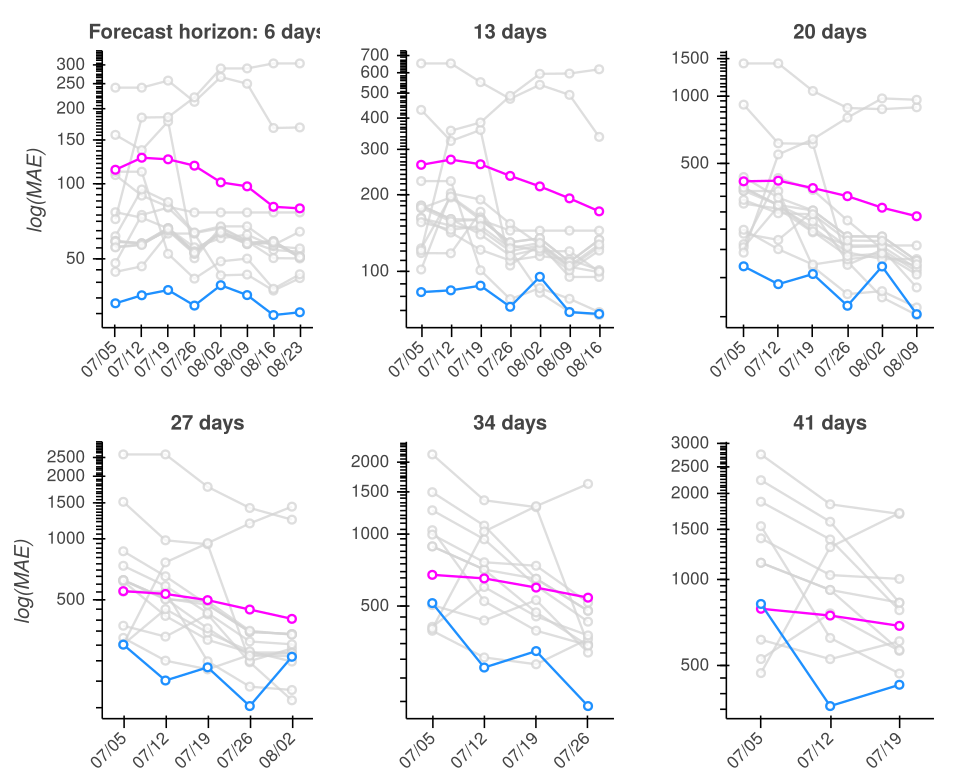
\includegraphics[width=\columnwidth]{img/us_mae_loss_ablation/us_mae_granger_ablation.png}
\caption{\label{fig:mae-covidhub-loss}Comparison of \bAR model with Negative Binomial (blue) and Poisson (magenta) likelihood. Forecast quality is measured in MAE.}
\end{figure}


\begin{marginfigure}[-4em]

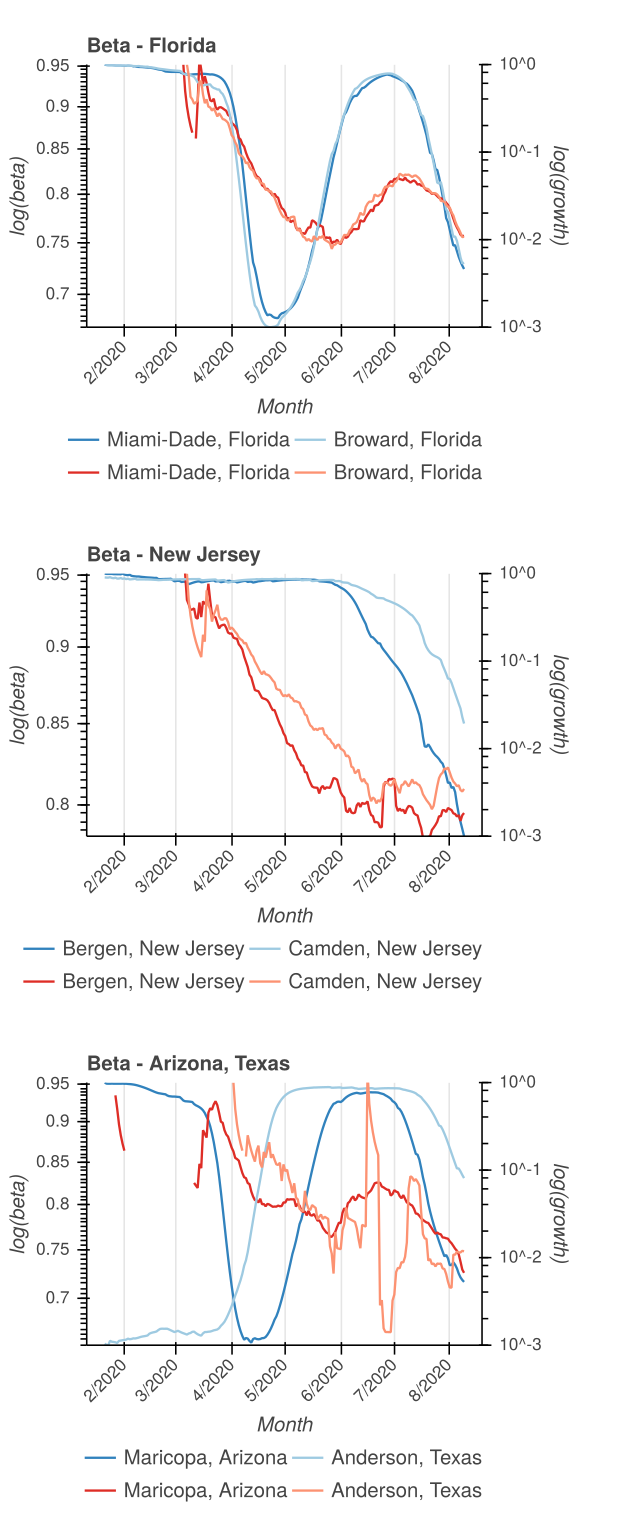
\includegraphics[width=\columnwidth]{img/betas.png}
\caption{Evolution of \(\beta\) over time}
\end{marginfigure}


In addition to county level case forecasts, we compare against state-level death forecasts from the Covid-19 Forecast Hub.  
MAE is computed using the Covid-19 Forecast Hub Evaluation script \sidenote[]{\url{https://github.com/youyanggu/covid19-forecast-hub-evaluation}}.
Models submitted to the forecast hub are released on different dates and have time horizons, so not all models have a prediction for each pair of dates.  
We've tried to pick dates that cover the most competitive models, and leave missing entries in the table indicated as " - ".  As can be seen from Table \ref{tab:state-deaths},
the \bAR model is quite competitive with other submissions, and has the lowest MAE for nearly half of all entires (9/19).

\begin{table*}
\centering
\begin{tabular}{lrrrrr}
\toprule
date & IHME-CurveFit & LANL-GrowthRate & UT-Mobility & YYG-ParamSearch & \bAR \\
2020-04-20 - 2020-05-09 & 388.1 & 327.9 & 519.4 & \cellcolor{red} 244.3 & 283.4 \\
2020-04-27 - 2020-05-16 & 455.8 & 271.7 & 461.3 & \cellcolor{red} 193.1 & 220.0 \\
2020-05-04 - 2020-05-23 & 139.0 & 164.1 & 393.3 & 125.2 & \cellcolor{red} 120.9 \\
2020-05-11 - 2020-05-30 &  -  & 151.4 & 200.0 & \cellcolor{red} 85.8 & 99.7 \\
2020-05-18 - 2020-06-06 & 144.2 & 107.8 & 205.1 & 107.9 & \cellcolor{red} 101.4 \\
2020-05-25 - 2020-06-13 &  -  & 100.0 & 134.0 & 111.3 & \cellcolor{red} 84.5 \\
2020-06-01 - 2020-06-20 &  -  & 98.2 & 134.0 & 107.5 & \cellcolor{red} 70.2 \\
2020-06-08 - 2020-06-27 & 128.8 & 125.1 & 135.8 & 105.2 & \cellcolor{red} 60.2 \\
2020-06-15 - 2020-07-04 & 130.2 &  -  & 131.6 & 109.5 & \cellcolor{red} 99.8 \\
2020-06-22 - 2020-07-11 & 120.5 &  -  & 132.1 & 125.1 & \cellcolor{red} 84.7 \\
2020-06-29 - 2020-07-18 & \cellcolor{red} 94.4 & 115.7 & 95.6 & 102.0 & 126.2 \\
2020-07-06 - 2020-07-25 & 141.7 & 144.8 & 147.6 & \cellcolor{red} 135.8 & 140.8 \\
2020-07-13 - 2020-08-01 &  -  & 179.3 & 118.4 & \cellcolor{red} 110.6 & 127.7 \\
2020-07-20 - 2020-08-08 &  -  & 196.9 & 146.4 & 122.1 & \cellcolor{red} 108.4 \\
2020-07-27 - 2020-08-15 &  -  & 220.7 & 232.0 & 118.9 & \cellcolor{red} 75.6 \\
2020-08-03 - 2020-08-22 &  -  & 179.3 & 358.2 & \cellcolor{red} 88.7 & 118.8 \\
2020-08-10 - 2020-08-29 &  -  & 118.5 &  -  & \cellcolor{red} 59.5 & 215.7 \\
2020-08-17 - 2020-09-05 &  -  & 111.3 & 177.7 & \cellcolor{red} 45.1 & 56.9 \\
2020-08-24 - 2020-09-05 & 108.1 & 61.0 & 61.4 & \cellcolor{red} 29.5 & 37.2 \\
\bottomrule
\end{tabular}
\vspace*{2em}
\caption{State Level Death Forecasts \label{tab:state-deaths}}
\end{table*}

\section{Related Work}
\label{sec:org4064e60}
We build on prior work that has proposed to use autoregressive models
for spatially and temporally aggregated disease surveillance data of endemic-epidemic
processes \citep{held2005statistical,meyer2014powerlaw,meyer2016socialcontact}.
Such autoregressive models are, for instance, used to monitor infectious
diseases by public health agencies like the Robert Koch Institute
\citep{salmon2016surveillance}.

Moreover, the negative binomial distribution has become a popular way to model
infectious diseases, largely to its ability to model count data with varying degrees
of overdispersion \citep{lloyd_smith2007negativebinomial}. Autoregressive models
in combination with negative binomial distributions have, for instance, been
used by \citet{bauer2018stratified,wakefield2019spatio,held2005statistical} to
model infectious disease count data.

\citet{valdes2005estimating} proposed a combination of VAR(1) models and \(\ell_1\)
regularization to for the discovery of Granger-causal relations to understand
brain connectivity. \citet{haufe2010sparse} proposed an improved estimator which
can be applied for VAR models of order \(p > 1\).

\section{Conclusion}
\label{sec:org29e484b}
To improve the quality and robustness of forecasts, we propose a new method
which aims to disentangle region-specific factors -- such as demographics,
enacted policies, and mobility -- from disease-inherent factors that influence
its spread. For this purpose, we combine recurrent neural networks with a vector
autoregressive model and train the joint model with a specific regularization
scheme that increases the coupling between regions. In our experiments, we
observe that our method achieves strong performance in predicting the spread of
COVID-19 when compared to state-of-the-art forecasts. Through ablations of the
model, we show that the relational approach in general, the added logit-normal
regularization, and the negative binomial likelihood are all important factors
that contribute to the forecast quality. Compared to existing state-of-the-art
forecasting models, our method takes a highly data-driven approach with fewer
modeling assumptions as, for instance, in very detailed and mechanistic
compartmental models. As such, we see our approach as complementary to existing
models with focus on strong forecasting performance at the cost of reduced
interpretability.



\newpage
\printbibliography
\end{document}
